% GNUPLOT: LaTeX picture with Postscript
\begingroup
  \makeatletter
  \providecommand\color[2][]{%
    \GenericError{(gnuplot) \space\space\space\@spaces}{%
      Package color not loaded in conjunction with
      terminal option `colourtext'%
    }{See the gnuplot documentation for explanation.%
    }{Either use 'blacktext' in gnuplot or load the package
      color.sty in LaTeX.}%
    \renewcommand\color[2][]{}%
  }%
  \providecommand\includegraphics[2][]{%
    \GenericError{(gnuplot) \space\space\space\@spaces}{%
      Package graphicx or graphics not loaded%
    }{See the gnuplot documentation for explanation.%
    }{The gnuplot epslatex terminal needs graphicx.sty or graphics.sty.}%
    \renewcommand\includegraphics[2][]{}%
  }%
  \providecommand\rotatebox[2]{#2}%
  \@ifundefined{ifGPcolor}{%
    \newif\ifGPcolor
    \GPcolorfalse
  }{}%
  \@ifundefined{ifGPblacktext}{%
    \newif\ifGPblacktext
    \GPblacktexttrue
  }{}%
  % define a \g@addto@macro without @ in the name:
  \let\gplgaddtomacro\g@addto@macro
  % define empty templates for all commands taking text:
  \gdef\gplbacktext{}%
  \gdef\gplfronttext{}%
  \makeatother
  \ifGPblacktext
    % no textcolor at all
    \def\colorrgb#1{}%
    \def\colorgray#1{}%
  \else
    % gray or color?
    \ifGPcolor
      \def\colorrgb#1{\color[rgb]{#1}}%
      \def\colorgray#1{\color[gray]{#1}}%
      \expandafter\def\csname LTw\endcsname{\color{white}}%
      \expandafter\def\csname LTb\endcsname{\color{black}}%
      \expandafter\def\csname LTa\endcsname{\color{black}}%
      \expandafter\def\csname LT0\endcsname{\color[rgb]{1,0,0}}%
      \expandafter\def\csname LT1\endcsname{\color[rgb]{0,1,0}}%
      \expandafter\def\csname LT2\endcsname{\color[rgb]{0,0,1}}%
      \expandafter\def\csname LT3\endcsname{\color[rgb]{1,0,1}}%
      \expandafter\def\csname LT4\endcsname{\color[rgb]{0,1,1}}%
      \expandafter\def\csname LT5\endcsname{\color[rgb]{1,1,0}}%
      \expandafter\def\csname LT6\endcsname{\color[rgb]{0,0,0}}%
      \expandafter\def\csname LT7\endcsname{\color[rgb]{1,0.3,0}}%
      \expandafter\def\csname LT8\endcsname{\color[rgb]{0.5,0.5,0.5}}%
    \else
      % gray
      \def\colorrgb#1{\color{black}}%
      \def\colorgray#1{\color[gray]{#1}}%
      \expandafter\def\csname LTw\endcsname{\color{white}}%
      \expandafter\def\csname LTb\endcsname{\color{black}}%
      \expandafter\def\csname LTa\endcsname{\color{black}}%
      \expandafter\def\csname LT0\endcsname{\color{black}}%
      \expandafter\def\csname LT1\endcsname{\color{black}}%
      \expandafter\def\csname LT2\endcsname{\color{black}}%
      \expandafter\def\csname LT3\endcsname{\color{black}}%
      \expandafter\def\csname LT4\endcsname{\color{black}}%
      \expandafter\def\csname LT5\endcsname{\color{black}}%
      \expandafter\def\csname LT6\endcsname{\color{black}}%
      \expandafter\def\csname LT7\endcsname{\color{black}}%
      \expandafter\def\csname LT8\endcsname{\color{black}}%
    \fi
  \fi
    \setlength{\unitlength}{0.0500bp}%
    \ifx\gptboxheight\undefined%
      \newlength{\gptboxheight}%
      \newlength{\gptboxwidth}%
      \newsavebox{\gptboxtext}%
    \fi%
    \setlength{\fboxrule}{0.5pt}%
    \setlength{\fboxsep}{1pt}%
\begin{picture}(4534.00,3400.00)%
    \gplgaddtomacro\gplbacktext{%
      \colorrgb{0.50,0.50,0.50}%
      \put(594,704){\makebox(0,0)[r]{\strut{}$0$}}%
      \colorrgb{0.50,0.50,0.50}%
      \put(594,1067){\makebox(0,0)[r]{\strut{}$20$}}%
      \colorrgb{0.50,0.50,0.50}%
      \put(594,1430){\makebox(0,0)[r]{\strut{}$40$}}%
      \colorrgb{0.50,0.50,0.50}%
      \put(594,1793){\makebox(0,0)[r]{\strut{}$60$}}%
      \colorrgb{0.50,0.50,0.50}%
      \put(594,2156){\makebox(0,0)[r]{\strut{}$80$}}%
      \colorrgb{0.50,0.50,0.50}%
      \put(594,2519){\makebox(0,0)[r]{\strut{}$100$}}%
      \colorrgb{0.50,0.50,0.50}%
      \put(726,484){\makebox(0,0){\strut{}$0$}}%
      \colorrgb{0.50,0.50,0.50}%
      \put(1408,484){\makebox(0,0){\strut{}$0.1$}}%
      \colorrgb{0.50,0.50,0.50}%
      \put(2090,484){\makebox(0,0){\strut{}$0.2$}}%
      \colorrgb{0.50,0.50,0.50}%
      \put(2773,484){\makebox(0,0){\strut{}$0.3$}}%
      \colorrgb{0.50,0.50,0.50}%
      \put(3455,484){\makebox(0,0){\strut{}$0.4$}}%
      \colorrgb{0.50,0.50,0.50}%
      \put(4137,484){\makebox(0,0){\strut{}$0.5$}}%
    }%
    \gplgaddtomacro\gplfronttext{%
      \csname LTb\endcsname%
      \put(220,1611){\rotatebox{-270}{\makebox(0,0){\strut{}Adversarial success (\%)}}}%
      \put(2431,154){\makebox(0,0){\strut{}$\epsilon$}}%
      \put(2431,3069){\makebox(0,0){\strut{}Black-box adversarial success using FGS samples from Model B }}%
      \put(2431,2849){\makebox(0,0){\strut{} on models trained with $ell_{infty}$ = 0.3 samples}}%
      \put(625,969){\makebox(0,0){\strut{}0.8}}%
      \csname LTb\endcsname%
      \put(796,971){\makebox(0,0){\strut{}0.9}}%
      \csname LTb\endcsname%
      \put(966,973){\makebox(0,0){\strut{}1.0}}%
      \csname LTb\endcsname%
      \put(1137,975){\makebox(0,0){\strut{}1.1}}%
      \csname LTb\endcsname%
      \put(1307,978){\makebox(0,0){\strut{}1.3}}%
      \csname LTb\endcsname%
      \put(1989,994){\makebox(0,0){\strut{}2.1}}%
      \csname LTb\endcsname%
      \put(2672,1163){\makebox(0,0){\strut{}11.4}}%
      \csname LTb\endcsname%
      \put(3354,2279){\makebox(0,0){\strut{}73.0}}%
      \csname LTb\endcsname%
      \put(4036,2456){\makebox(0,0){\strut{}82.7}}%
      \csname LTb\endcsname%
      \put(3150,1537){\makebox(0,0)[r]{\strut{}iterative}}%
      \csname LTb\endcsname%
      \put(625,970){\makebox(0,0){\strut{}0.8}}%
      \csname LTb\endcsname%
      \put(796,975){\makebox(0,0){\strut{}1.1}}%
      \csname LTb\endcsname%
      \put(966,979){\makebox(0,0){\strut{}1.3}}%
      \csname LTb\endcsname%
      \put(1137,983){\makebox(0,0){\strut{}1.6}}%
      \csname LTb\endcsname%
      \put(1307,988){\makebox(0,0){\strut{}1.8}}%
      \csname LTb\endcsname%
      \put(1989,1023){\makebox(0,0){\strut{}3.7}}%
      \csname LTb\endcsname%
      \put(2331,1053){\makebox(0,0){\strut{}5.4}}%
      \csname LTb\endcsname%
      \put(2672,1220){\makebox(0,0){\strut{}14.6}}%
      \csname LTb\endcsname%
      \put(3013,2018){\makebox(0,0){\strut{}58.5}}%
      \csname LTb\endcsname%
      \put(3354,2285){\makebox(0,0){\strut{}73.3}}%
      \csname LTb\endcsname%
      \put(3695,2406){\makebox(0,0){\strut{}80.0}}%
      \csname LTb\endcsname%
      \put(4036,2477){\makebox(0,0){\strut{}83.8}}%
      \csname LTb\endcsname%
      \put(3150,1317){\makebox(0,0)[r]{\strut{}standard}}%
      \csname LTb\endcsname%
      \put(625,970){\makebox(0,0){\strut{}0.8}}%
      \csname LTb\endcsname%
      \put(796,972){\makebox(0,0){\strut{}0.9}}%
      \csname LTb\endcsname%
      \put(966,974){\makebox(0,0){\strut{}1.1}}%
      \csname LTb\endcsname%
      \put(1137,975){\makebox(0,0){\strut{}1.1}}%
      \csname LTb\endcsname%
      \put(1307,974){\makebox(0,0){\strut{}1.1}}%
      \csname LTb\endcsname%
      \put(1989,979){\makebox(0,0){\strut{}1.3}}%
      \csname LTb\endcsname%
      \put(2331,988){\makebox(0,0){\strut{}1.8}}%
      \csname LTb\endcsname%
      \put(2672,1011){\makebox(0,0){\strut{}3.1}}%
      \csname LTb\endcsname%
      \put(3013,1296){\makebox(0,0){\strut{}18.8}}%
      \csname LTb\endcsname%
      \put(3354,2105){\makebox(0,0){\strut{}63.4}}%
      \csname LTb\endcsname%
      \put(3695,2390){\makebox(0,0){\strut{}79.1}}%
      \csname LTb\endcsname%
      \put(4036,2474){\makebox(0,0){\strut{}83.7}}%
      \csname LTb\endcsname%
      \put(3150,1097){\makebox(0,0)[r]{\strut{}ensemble}}%
      \csname LTb\endcsname%
      \put(625,969){\makebox(0,0){\strut{}0.8}}%
      \csname LTb\endcsname%
      \put(796,979){\makebox(0,0){\strut{}1.3}}%
      \csname LTb\endcsname%
      \put(966,995){\makebox(0,0){\strut{}2.2}}%
      \csname LTb\endcsname%
      \put(1137,1022){\makebox(0,0){\strut{}3.7}}%
      \csname LTb\endcsname%
      \put(1307,1071){\makebox(0,0){\strut{}6.4}}%
      \csname LTb\endcsname%
      \put(1989,1681){\makebox(0,0){\strut{}40.0}}%
      \csname LTb\endcsname%
      \put(2331,1983){\makebox(0,0){\strut{}56.6}}%
      \csname LTb\endcsname%
      \put(2672,2158){\makebox(0,0){\strut{}66.3}}%
      \csname LTb\endcsname%
      \put(3013,2284){\makebox(0,0){\strut{}73.2}}%
      \csname LTb\endcsname%
      \put(3354,2381){\makebox(0,0){\strut{}78.6}}%
      \csname LTb\endcsname%
      \put(3695,2445){\makebox(0,0){\strut{}82.1}}%
      \csname LTb\endcsname%
      \put(4036,2491){\makebox(0,0){\strut{}84.6}}%
      \csname LTb\endcsname%
      \put(3150,877){\makebox(0,0)[r]{\strut{}no adv.}}%
    }%
    \gplbacktext
    \put(0,0){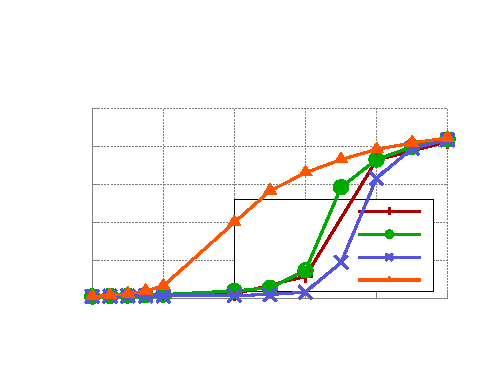
\includegraphics{latex_plots/modelB_to_modelA(0.3)_all}}%
    \gplfronttext
  \end{picture}%
\endgroup
